\graphicspath{{chapters/06/images6/}}
\chapter{Gene set enrichment}
	\section{Introduction}
	The aim is to go from differentially expressed genes found in previous analyses to biological functions. How does my data relate to known biological functions? Are there specific functions that are characterized by gene expression changes?

	\subsection{Functional groups characterized by gene expression change}
	Functional groups characterized by gene expression change are:

	
		\begin{itemize}
			\item \textbf{Gene sets}: the set is scored depending on the expression level of its member genes. It will be discussed in section \ref{sec:genesets}
			\item \textbf{Network}: they can be just visual, identify modules satisfying some joint gene expression and topology requirement.
			\item \textbf{Pathways}: they can be just visual, or they are scored exploiting gene expression and topology.
		\end{itemize}

Before diving into the concepts od GSE, we will first have a look at Gene Ontology.
	



%%%%%%%%%%%%%%%%%%%%%%%%%%%%%%%%%%%%%%%%%%%%%%%%%%%%%%%%%%%%%%%%%%%%%%%%%%%%%%%%%%%%%%%%%%%%%%%%%%%
	\section{Gene Ontology}
	An \textbf{ontology} formally represents knowledge as a set of concepts within a domain and the relationships among those concepts.
	It can be used to reason about the entities within that domain and may be used to describe the domain.
	A \textbf{controlled vocabulary} provides a way to organize knowledge for subsequent retrieval, but does not allow reasoning about the entities.
Ontologies and controlled vocabularies are heavily used in biological databases as they allow the organization of data within a database, providing a meaningful link between databases structure and search queries.

\section{Gene ontology}
A gene ontology is a way to capture biological knowledge for individual gene products in a written and computable form, in the sense that it has a formal structure such that it can be used by a machine.
A GO can also be defined as a set of concepts and their relationships to each other is arranged as a hierarchy.
An ontology is structured as an acyclic graph where terms can have more than one parent (figure \ref{fig:GO}).
	Terms are linked by directed relationships like: "is part of", "regulates".
	Each node can have multiple parents, but no cycles. 
	
\begin{figure}
\centering
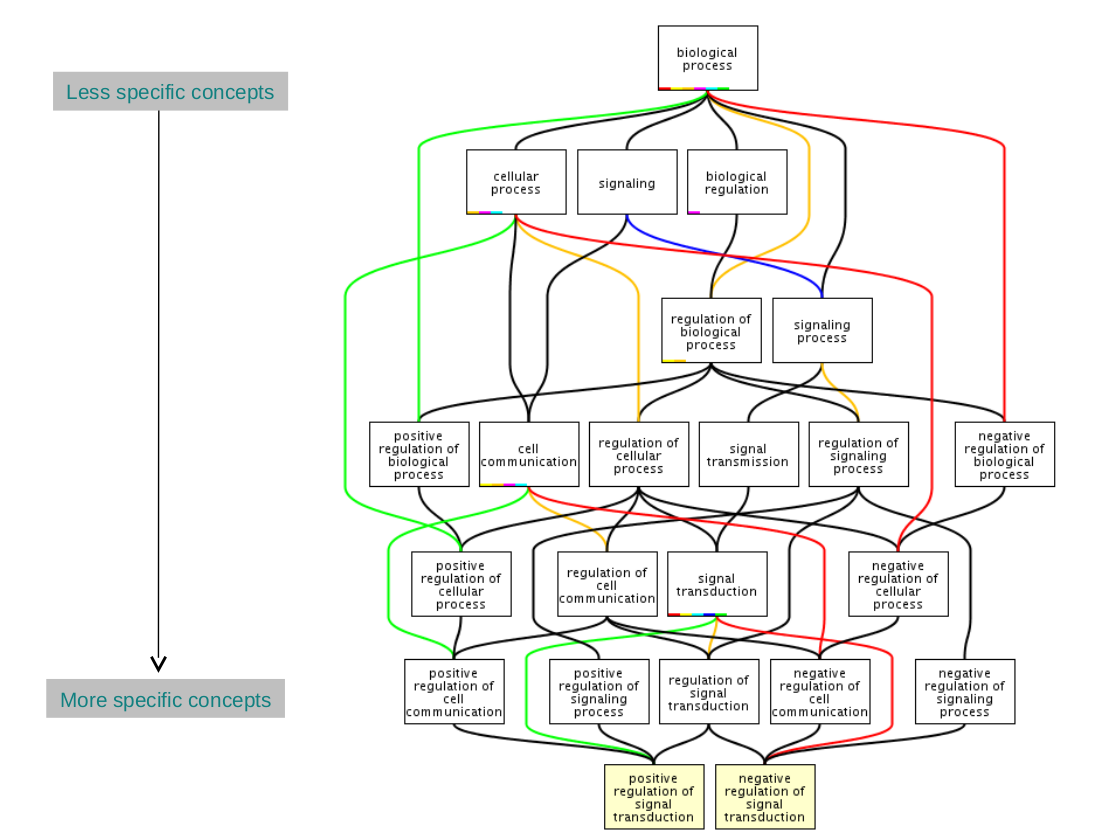
\includegraphics[scale=0.35]{GO}
\caption{Acyclic graph representation of Gene Ontology}
\label{fig:GO}
\end{figure}

\subsection{Concepts in GO}
GO is organized in three main hierarchies:
\begin{itemize}
\item Molecular Function: an elemental activity, task or job (e.g., protein kinase activity);
\item Biological Process: a commonly recognized series of events (e.g., cell division);
\item Cellular Component: where a gene product is located (e.g. mitochondrion).
\end{itemize}

Each one of these has its own acyclic graph which contains a detailed description of the biological domain focusing on these three different abstraction levels. 

		\subsubsection{Molecular Function}
		The molecular function describes \textbf{activities} that happen at a molecular level like catalytic or binding activity.
		This category includes the activities rather than the entities that are involved in an action and do not specify where, when or in which context the actions happen.
		Molecular functions can be executed by single gene products or complexes of gene products.
		Some examples are:

		\begin{multicols}{4}
			\begin{itemize}
				\item Catalytic activity;
				\item Transport activity;
				\item Binding;
				\item Toll receptor binding (more specific).
			\end{itemize}
		\end{multicols}

		\subsubsection{Biological process}
		A biological process is a series of events resulting from multiple ordered groups of molecular functions.
		A biological process is different from a pathway, as gene ontology does not report the dynamics or the dependencies that are required to describe a pathway.
		Some examples are:

		\begin{multicols}{4}
			\begin{itemize}
				\item Cellular physiological processes.
				\item Signal transduction.
				\item Metabolic process of pyrimidine.
				\item Glucose transport.
			\end{itemize}
		\end{multicols}
		It might be difficult to distinguish between molecular functions and biological processes.
		A general rule is that a process should include multiple distinct passages.

		\subsubsection{Cellular component}
		A cellular component is linked to a component of a cell with the condition that is part of a larger object and can be part of an anatomic structure.
		Some examples are:

		\begin{multicols}{4}
			\begin{itemize}
				\item Ribosome.
				\item Nucleus.
				\item Neuron parts.
				\item Internal nuclear membrane.
			\end{itemize}
		\end{multicols}
		

	\subsection{The gene ontology project}
	Originally in the gene ontology or GO project the hierarchies were completely independent, without links between them.
	From $2009$ biological processes and molecular functions are \textbf{linked}, as biological processes are ordered assemblies of molecular functions.
	GO is required as there are inconsistencies in the human language: different concepts can have the same name.
	Furthermore it enables to interpret quickly large datasets.
	The aim of the GO project is to:

	\begin{multicols}{3}
		\begin{itemize}
			\item Compile ontologies.
			\item Annotate gene products using ontology terms.
			\item Provide a public resource of data and tools for annotation.
		\end{itemize}
	\end{multicols}

	A gene ontology annotation is a statement that a gene product has a particular molecular function (or is involved in a particular biological process, or is located within a certain cellular component), determined by a particular method and described in a reference.
	
	
	
	
	

\section{Gene-set Enrichment Analysis}\label{sec:genesets}
	Gene-set enrichment analysis is the breakdown of cellular functions into gene sets.
	Every set of gene is associated to a specific cellular:

	\begin{multicols}{4}
		\begin{itemize}
			\item Function.
			\item Process.
			\item Component.
			\item Pathway.
		\end{itemize}
	\end{multicols}

	Microarray or RNA-seq data can be related to gene sets in order to mine its functional meaning, to find which gene-sets \textbf{summarize at best} gene expression patterns.

	\subsection{Sources and types}
	Other than Gene Ontology there are other sources and types of gene-sets:

		\begin{itemize}
			\item Pathways (KEGG).
			\item Protein families and domains (PFAM).
			\item Predicted target of regulators like mRNA and transcription factors (MSigDB-c3).
			\item Protein-protein interaction modules.
			\item Gene expression:

				\begin{itemize}
					\item Up and down regulation after treatment or in relation to disease (MSigDB-c2).
					\item Co-expression across many conditions (MSigDB-c4).
				\end{itemize}

			\item Genotype-phenotype association (DiseaseHub).
			\item Genomic position (MSigDB-c1).
		\end{itemize}

		The main resources for this type of data are:
	
			\begin{itemize}
				\item Bioconductor.
				\item DiseaseHub.
				\item MSigDB.
				\item PathwayCommons.
				\item WhichGenes.
			\end{itemize}
		

	\subsection{Differences between pathways and processes}
	From a biological perspective the difference between pathways and processes is philosophical.
	It is still worth speculating in a bioinformatics perspective because a gene is annotated for a GO biological process if the curators deem it significantly contributes to the process according to a number of evidences.
	Pathway include the wiring of genes and gene products, hence they rely on a more intensive curation process.
	Some pathways include large ubiquitous actors such as the proteasome that may confound enrichment analysis, whereas the are usually absent from GO processes.
	
	
	\subsection{Enrichment methods}
	An enrichment test combines a gene expression matrix with gene-set databases to build an enrichment table.
	In the enrichment table each gene set is associated with a p-value, that gives use the probability that the differentially expressed genes are part of the gene set.
	This is a two class design: genes can be ranked according to different statistics like fold change, log ratio or t-test and a selection by threshold can be performed.
	Other designs can be implemented, for example an expression matrix can be obtained with multiple conditions employing for example ANOVA.
	\\
	After choosing which genes are down- and up-regulated form the gene expression table (or matrix), the actual enrichment test can be performed. 
	A gene set can both overlap with significant gene and background genes.
	To test whether this overlap is significant it must be compared with random sampling of captured genes.
	If by repeating the random sampling we never find a bigger overlap than the one we selected, it means that the gene-set is not casual.

		\subsubsection{Fisher's exact test}
		
		\begin{figure}
		\centering
		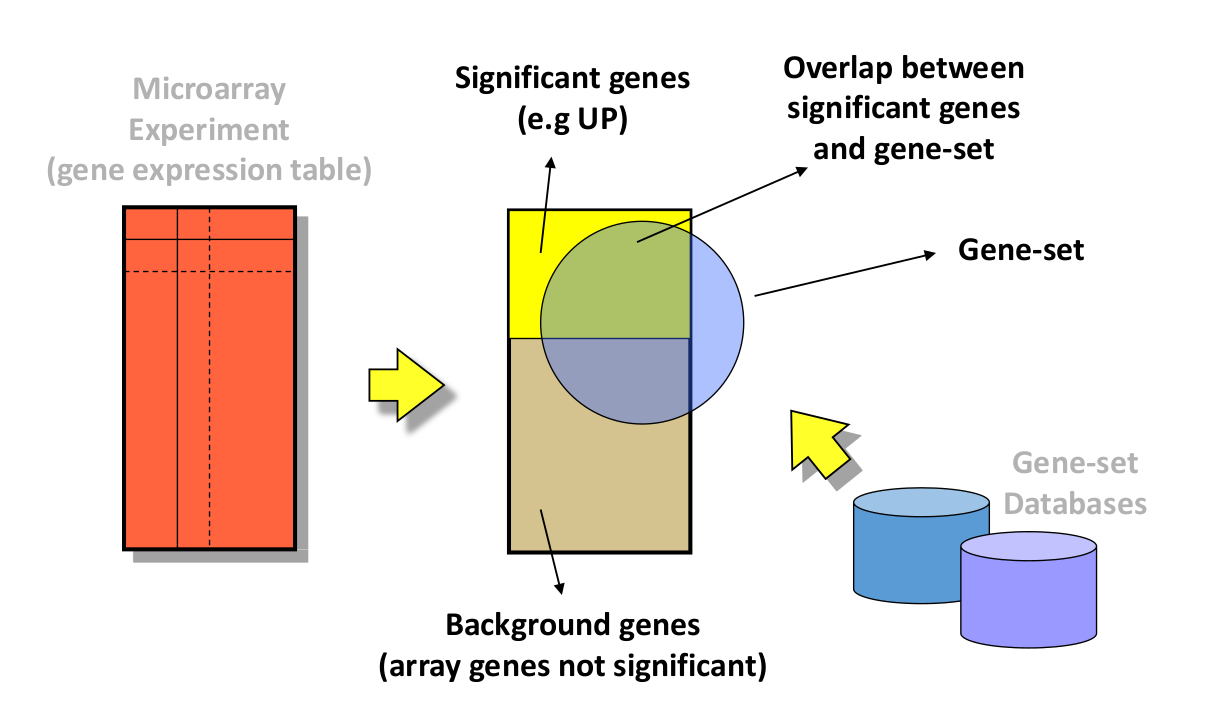
\includegraphics[scale=0.2]{test_microarray}
		\caption{In this microarray two-class experimental design, significant genes are selected by a threshold. The circle represents the overlap between significant genes and gene-set. Fisher's test will test if this overlap is larger than expected by random sampling the captured genes?}
		\label{fig:test-microarray}
\end{figure}				
		
		Fisher's exact test calculates the exact probability of the table of observed cell frequencies in a table given that:

			\begin{itemize}
				\item The null hypothesis of independence is true.
				\item The marginal totals of the observed table are fixed.
			\end{itemize}

		It does not require to perform random sampling as it is based on the theoretical null-hypothesis distribution: the hypergeometric distribution.
		In particular it gives the probability that the overlap between significant genes and gene-set is greater than the one expected by random sampling the captured genes.
		Fisher's table is built such that:

		\begin{table}[H]
			\centering
			\begin{tabular}{ccccc}
				\multirow{4}{*}{\rotatebox[origin=c]{90}{\tiny{Up regulated genes}}}& \multicolumn{4}{c}{Gene Set}\\
				 & & No & Yes & \\
				 \cline{3-4}
				 &Yes & \multicolumn{1}{|c|}{$a$} & \multicolumn{1}{|c|}{$b$} & $a+b$\\
				 \cline{3-4}
				 &No & \multicolumn{1}{|c|}{$c$} & \multicolumn{1}{|c|}{$d$} & $c+d$\\
				 \cline{3-4}
				 & & $a+c$ & $b+d$ & \\
			\end{tabular}
			\caption{Fisher's exact test table}
			\label{tab:fisher}
		\end{table}

		Considering the table \ref{tab:fisher}, $a$, $b$, $c$, $d$ are the size of the four subsets.:

			\begin{itemize}
				\item $a$ significant genes not in overlap.
				\item $b$ significant genes not in overlap.
				\item $c$ background genes in overlap.
				\item $d$ background gene in overlap.
			\end{itemize}
		
		With "significant" meaning down- or up-regulated, based on our experimental design.
		Then the exact probability of the table is:

		$$\frac{(a+b)!\cdot(c+d)!\cdot(a+c)!\cdot(b+d)!}{n!\cdot a!\cdot b!\cdot c!\cdot d!}$$

		The p-value is calculated by summing all probabilities less than or equal to the probability of the observed table.
		Fisher's exact test can be used to evaluate the overlaps between gene-sets from databases.
		It is usually employed in threshold-dependent scenario and suffers from some limitations.

	\subsection{Whole-distribution - GSEA enrichment}
	Enrichment test can either be threshold-dependent, e.g., Fisher's test, but can also  be a \textbf{whole-distribution} test, e.g. GSEA, which considers all the genes in the experiment.
	
	\begin{figure}[H]
	\centering
	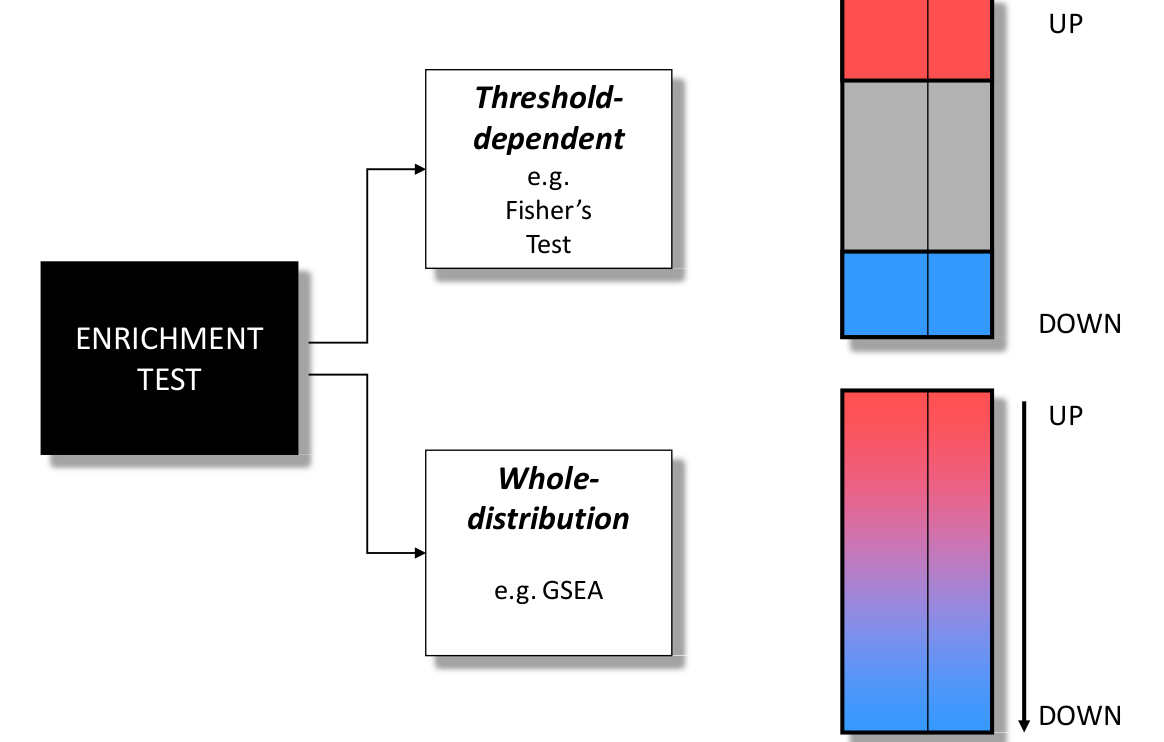
\includegraphics[scale=0.2]{beyond}
	\caption{Difference between an enrichment test with genes selected by a threshold \textit{vs} GSEA }
	\label{fig:beyond}
	\end{figure}
	
	Whole distribution methods like GSEA, gene set enrichment analysis, have been shown to be more stable and statistically powerful.
	Instead of excluding genes they are ranked according to a measure.
	
	GSEA is useful as it tackles three major threshold methods' problems:
	\begin{itemize}
	\item There is no "natural" value for the threshold;
	\item Different results at different threshold settings;
	\item Loss of information due to thresholding (No resolution between significant signals with different strengths, weak signals neglected)
	\end{itemize}
	
	GSEA can work on two different experimental designs.
	It can either use the expression matrix of a two-class comparison and rank the genes based on fold change, log-ratio, t-test and SAM; but it can also use the expression matrix of \textbf{correlation to phenotype}: in this case the genes will be ranked based on the Pearson correlation.
	We will be focusing on the two-class comparison experimental design.

		\subsubsection{Process}
		\begin{description}
		\item[Calculate the ES score]
		First the enrichment score is calculated: genes are ranked according to a specific measure like the fold change.
		It tells us where are the gene-set genes located in the ranked list and if the distribution is random, or if there's an enrichment in either end.
		
		Then the chance of observing a gene in a position towards the upregulated or down-regulated region is computed.
		Based on the position in which genes are found, it can be established whether the event is random or not.
		Every gene present in a gene list gives a positive contribution, while every absent one a negative one.
		
		The final ES score is the maximum running ES score.
		
		So, an high enrichment score means high local enrichment, and vice versa.
		
		To state that there's an enrichment we need to compare the ES againts a null hypothesis. 
		In Fisher's test the test itself provided a p-value, in this case the p-value is calculated using a permutation method.
		
		
		\begin{figure}[H]
	\centering
	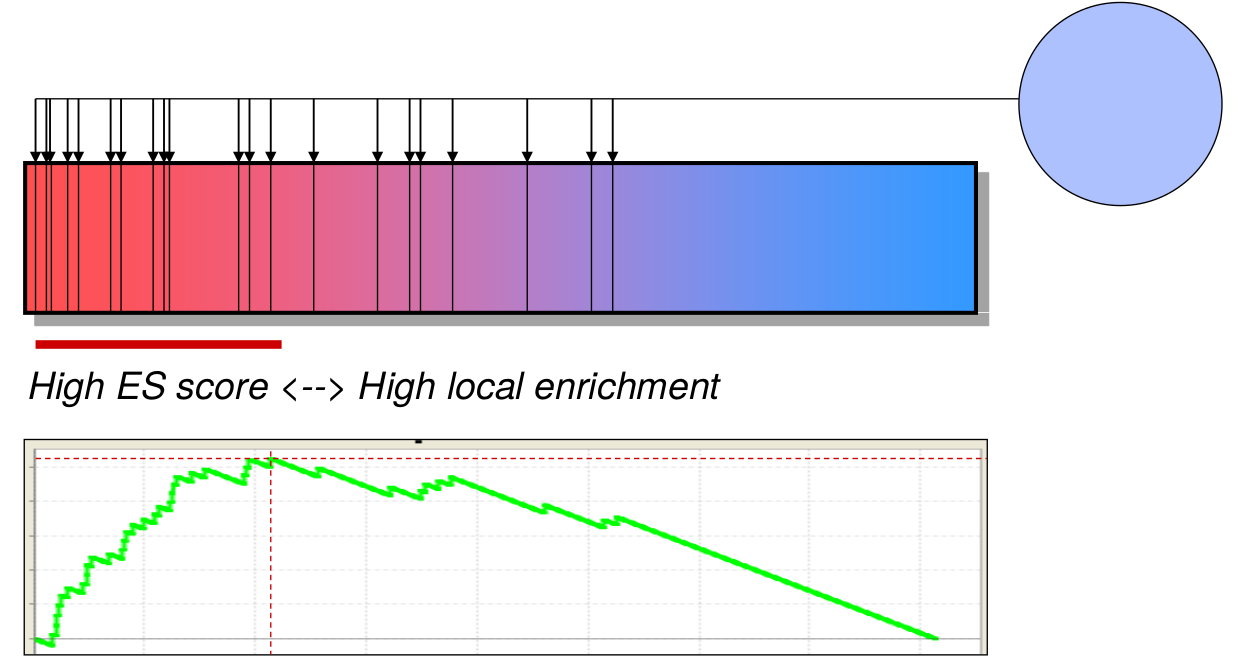
\includegraphics[scale=0.2]{method1}
	\caption{Top bar: Indicates where the gene-set genes are located in the ranked list. We need to find out whether the distribution random, or if there's an enrichment in either end.
	Every present gene (black vertical bar) gives a positive contribution, while every absent gene (no vertical bar) gives a negative contribution. 
	\\
	Bottom graph: The bottom curve is the running ES score.}
	\label{fig:method1}
	\end{figure}
	
		\item[Empirical p-value estimation]
		We need a way to estimate the empirical p-value for every gene-set.
			\begin{itemize}
			\item From randomized data a null-hypothesis distribution is generated. See permutation setting in subsection \ref{subsub:perm}!
			\item The empirical p-value is computed observing how many random data have enrichment score greater than the read ones.
		The p-value is estimated for each gene set for which we calculated the ES.
			\end{itemize}
		
		\begin{figure}[H]
	\centering
	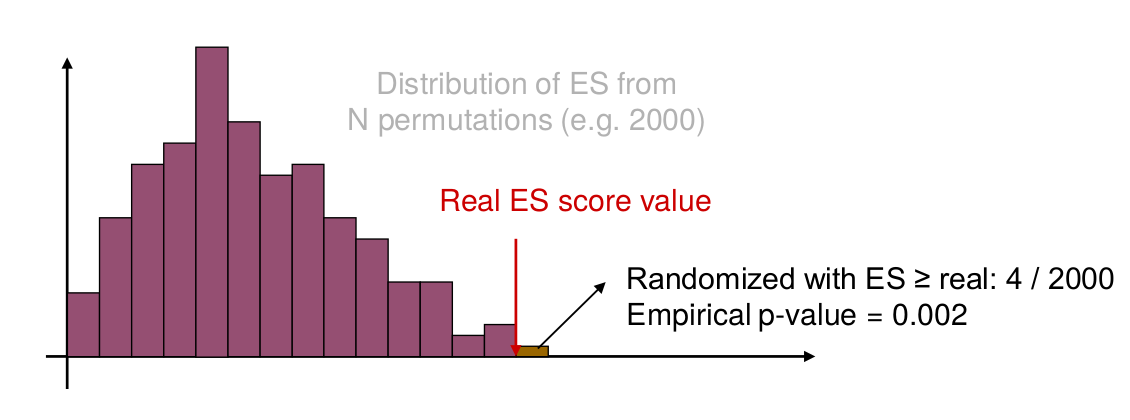
\includegraphics[scale=0.2]{method2}
	\caption{Estimation of the empirical p-value for each gene-set}
	\label{fig:method1}
	\end{figure}
		
		\item[Calculate the FDR - False Discovery Rate correction]
		
			Then the FDR correction of the p-value is computed.
		The standard ranking metrics is:

		$$\log_2 FC\cdot -10\log_{10} pvalue$$
		
		\end{description}
		
		N.B.: The p-value only depends on the single gene-set performance, while the FDR depends on the performance of all gene-sets.

		\subsubsection{Permutations}\label{subsub:perm}
		Permutations setting have important implications.
		\textbf{Gene permutations} can be used when biological replicates are very similar within classes and classes are well separated
		When biological replicates tend to be dissimilar or stratified according to hidden experimental factors \textbf{other whole-distribution enrichment methods} need to be used.

		\subsubsection{Other uses of GSEA}
		The GSEA tool allow to perform more general types of analysis specifying designs:
		
			\begin{itemize}
				\item .GMT data format contains GO ID, description and information of the genes contained in the GO term.
				\item The gene expression table contains CDM or RPKM values for each gene.
				\item The expression phenotype file .cls determine which sample belongs to which class.
			\end{itemize}


	\subsection{Gene set filter}
	Gene set for enrichment analysis are usually filtered by size.
	Large gene-sets are undesired if they are derived from gene ontology or other functional resources as the usually correspond to uninformative concepts (e.g., regulation of biopolymer catabolism).
	Small gene-sets are undesired as their statistics are noisy and may decrease the FDR of other sets.

	\subsection{Redundancy problem}
	There are many redundant gene-sets.
	For example gene ontology has a very large number of gene-sets, often with slight differences.
	Moreover different pathway databases have different but overlapping definitions of pathways.
	Globally it is useful to grasp the overlap relations between enriched gene-sets.
	To do so a visualization framework beyond the enrichment table is needed.
	The redundancy problem can be handled by correcting for inter-redundancy and prioritizing the most enriched gene-sets or by visualizing gene-set overlap as a network with the EnrichMap tool.
	Considering up and down regulation a map can be built such that:

		\begin{itemize}
			\item Each node is a gene set.
			\item The color represent differentially expressed genes.
			\item The size of the node is the number of genes.
			\item The edge thickness the overlap or similarity degree.
		\end{itemize}
	
	The network can be then clustered based on similarity values in order to identify redundancy sets.
